\section{Spatial Graph Diagrams}

\subsection{Reidemeister Moves}

\subsubsection{Reidemeister 1}

## Reidemeister 1

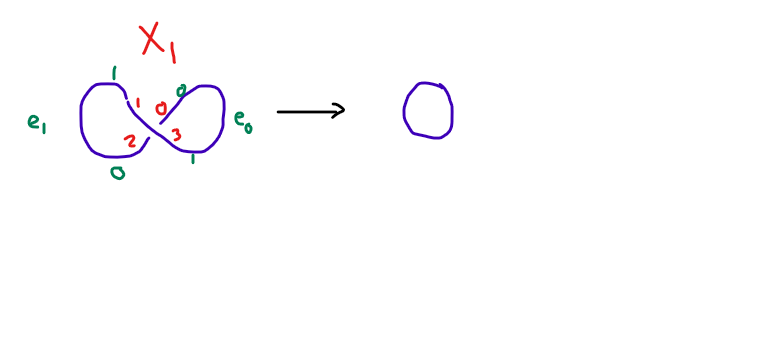
\includegraphics[scale=0.5]{test_spatial_graph_diagrams/images/r1_1}
\lstinputlisting[linerange={5-22}]{test_spatial_graph_diagrams/test_R1_move.py}

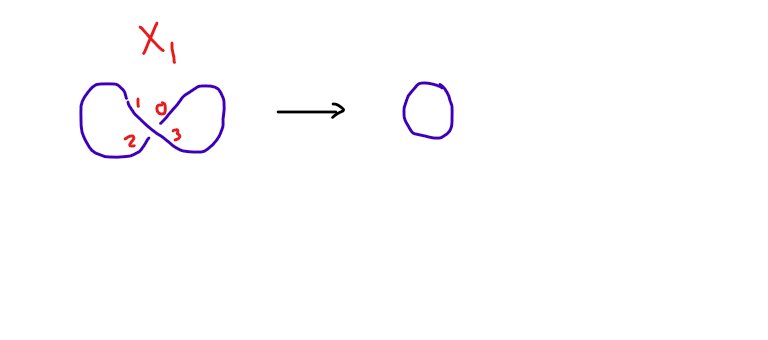
\includegraphics[scale=0.5]{test_spatial_graph_diagrams/images/r1_2}
\lstinputlisting[linerange={36-59}]{test_spatial_graph_diagrams/test_R1_move.py}

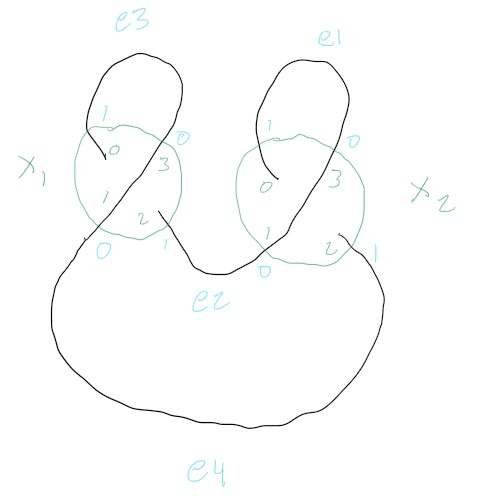
\includegraphics[scale=0.5]{test_spatial_graph_diagrams/images/r1_double_loop_same_orientation}

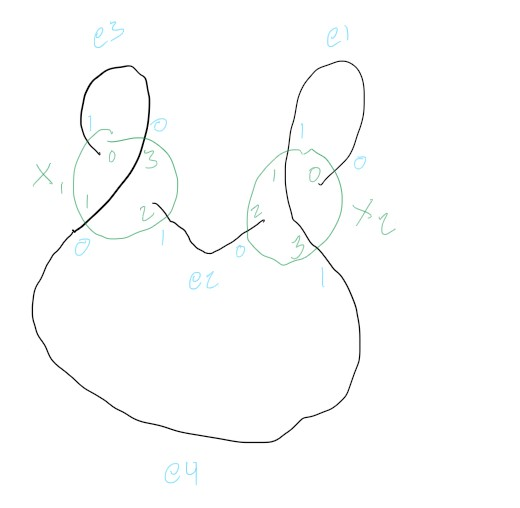
\includegraphics[scale=0.5]{test_spatial_graph_diagrams/images/r1_double_loop_opposite_orientation}


\subsubsection{Reidemeister 2}

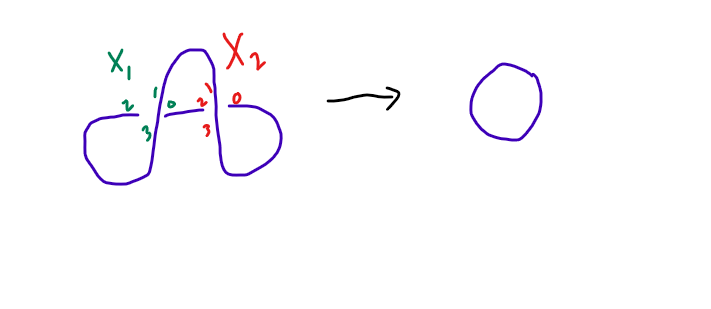
\includegraphics[scale=0.5]{test_spatial_graph_diagrams/images/r2_1}

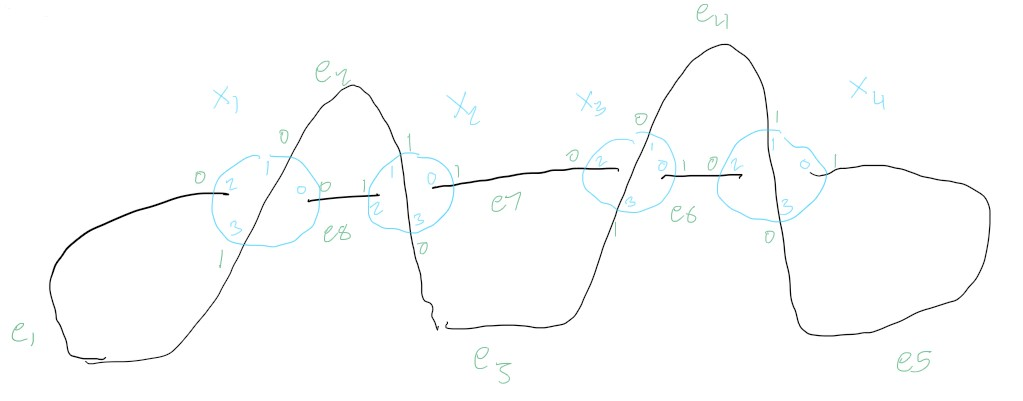
\includegraphics[scale=0.5]{test_spatial_graph_diagrams/images/r2_double_loop_same}

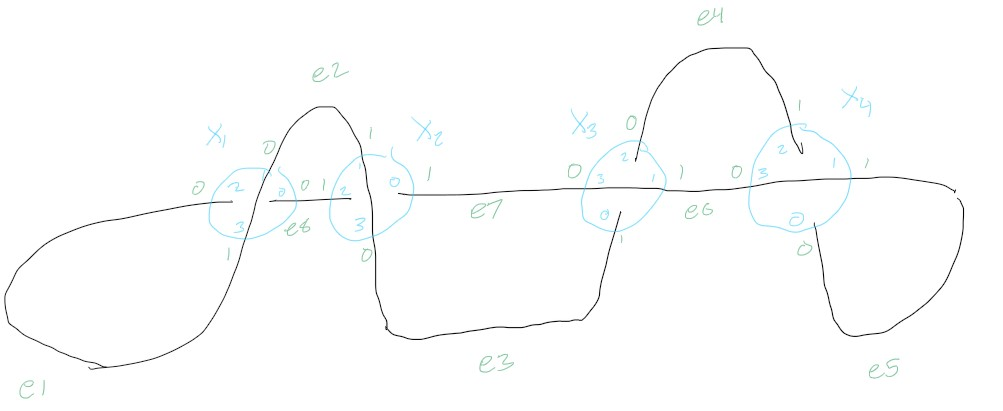
\includegraphics[scale=0.5]{test_spatial_graph_diagrams/images/r2_double_loop_opposite}



\subsubsection{Reidemeister 3}

# The Reidemeister 3 Move

# Prerequisites:
1. The SGD has at least one face whose 3 vertices are crossings.
2. The candidate face has at least one edge that pass completely under or over the other two edges.


# Algorithm:
1. Identify the candidate face for the R3 move.
    - If there is more than one face that satisfies the R3 prerequisites, then choose one (TODO Implement choosing logic).

2. Identify the candidate edge for the R3 move.
    - If the chosen face as more than one edge that passes completely under or over the other two edges, choose one (TODO Implement choosing logic).

3. Label each vertex and edge of the candidate face.
    - The R3 moves one edge across its opposing vertex.
    - The chosen edge will be called the "moving" or "opposite" edge since it will move across the opposing vertex.
    - The vertex opposing the moving edge will be called the "keep" crossing since it will remain in place.
    - The two edges adjacent to the keep crossing will be called "common" edges (as opposed to the opposing edge).
    - The two other crossings will be called "remove" crossings since moving the opposite edge will remove these crossings (and introduce two new crossings on the other side of the keep crossing).

4. Identify how edge and crossing indices will change by the R3 move.
    - The moving edge intersects with two keep crossing edges. The R3 move will cause it to intersect the opposite two edges (i... ).
    - When we remove the two remove crossings, two edges represent the moving edge and will be moved by the R3 move. The other two edges must spliced together.
    - ...

5. Perform the R3 move.
    - Delete the two edges that do not move.
    - Connect ...
    - Shift the two move crossings
    - Add new edges...
    -

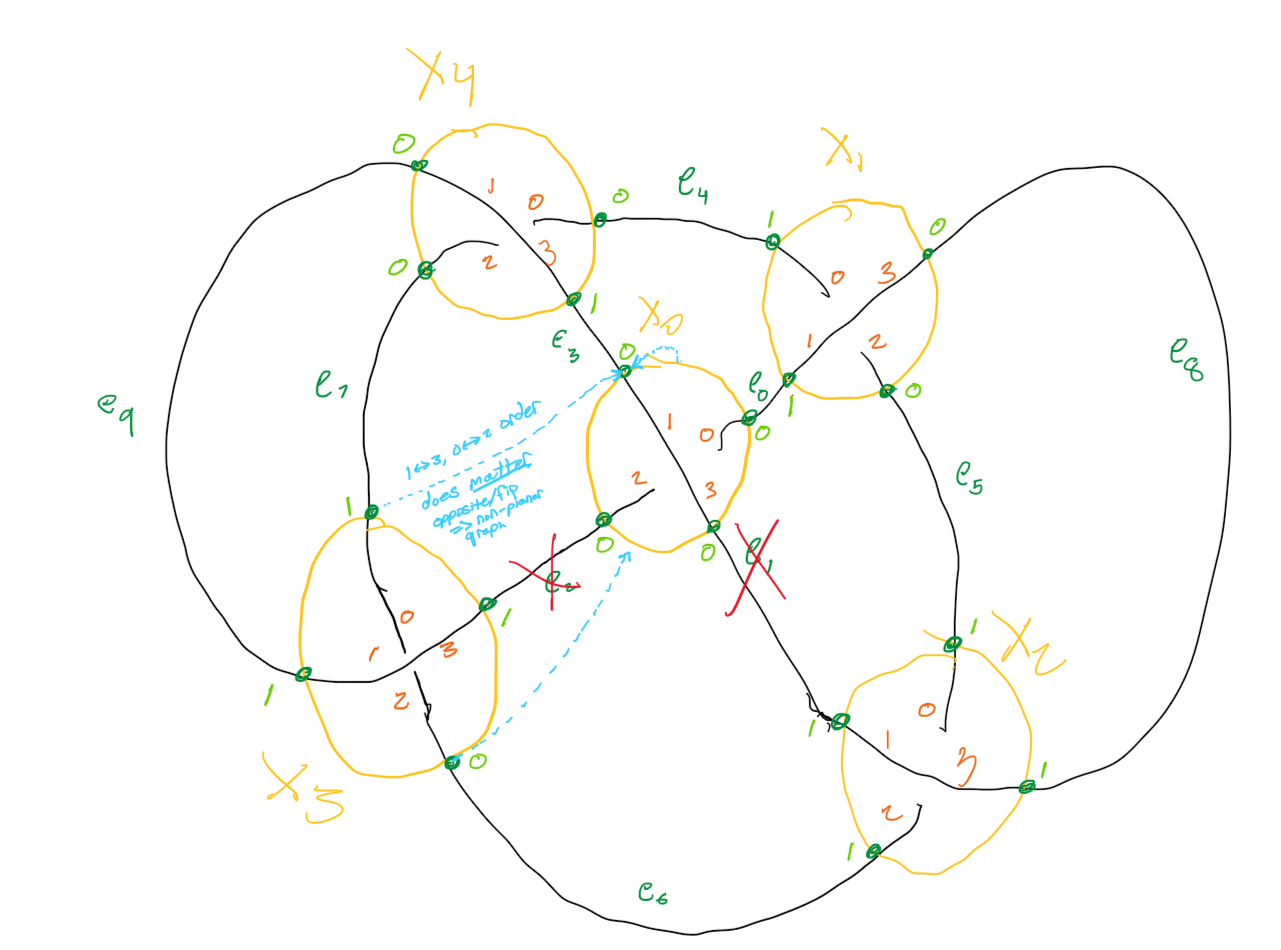
\includegraphics[scale=0.5]{test_spatial_graph_diagrams/images/r3_before_move}

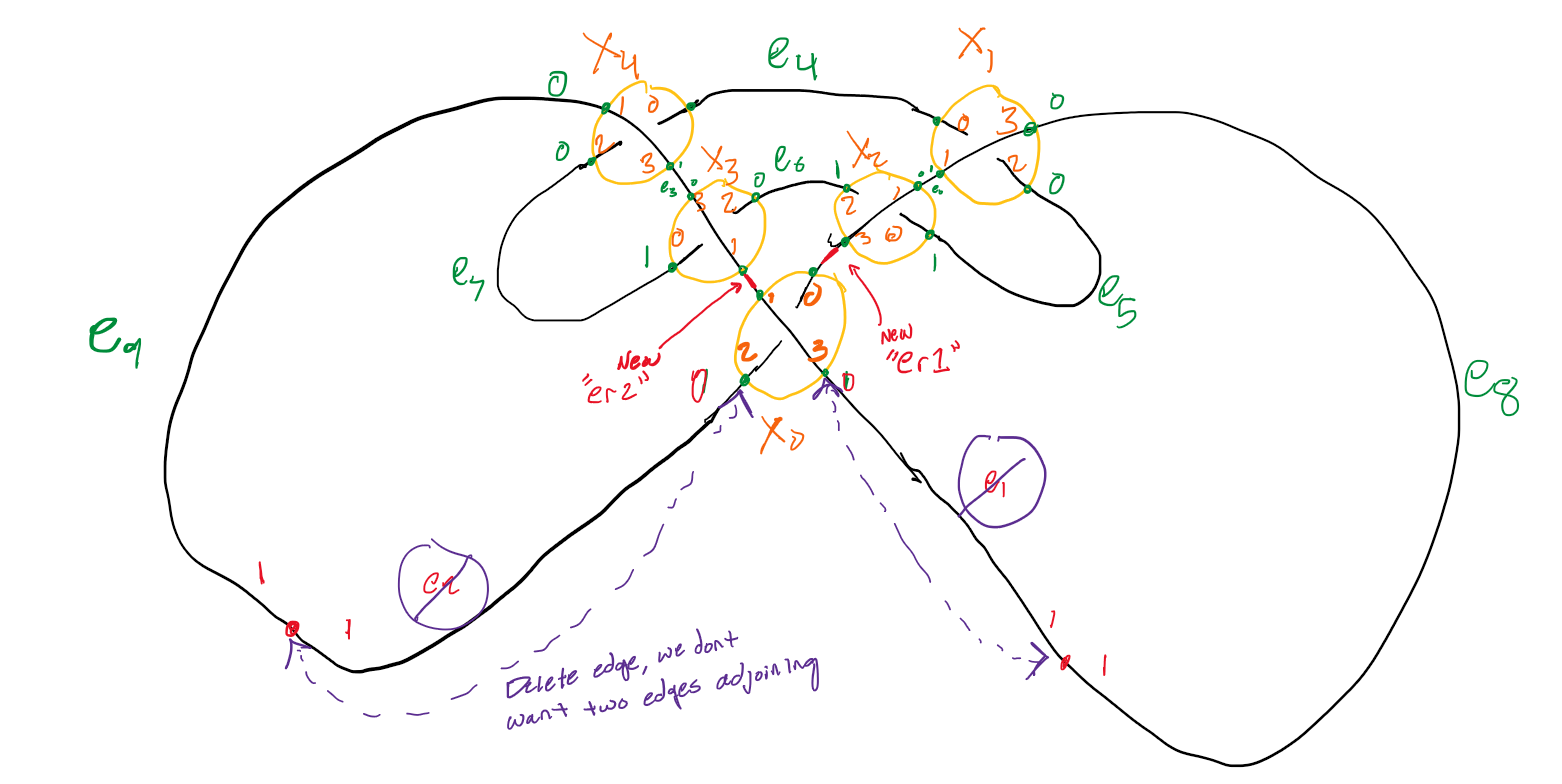
\includegraphics[scale=0.5]{test_spatial_graph_diagrams/images/r3_after_move}


\subsubsection{Reidemeister Simplification}